%----------------------------------------------------------------------------------------
%	PACKAGES AND OTHER DOCUMENT CONFIGURATIONS
%----------------------------------------------------------------------------------------

\documentclass{article} % paper and 12pt font size
\usepackage{amsmath,amsfonts,amsthm} % Math packages
\usepackage[margin=1in]{geometry}
\usepackage[ruled,vlined]{algorithm2e}
\usepackage{graphicx}
\usepackage{tabu}
\usepackage{float}
\usepackage[parfill]{parskip}
\usepackage[labelsep=quad,indention=10pt]{subfig}
\setlength{\paperwidth}{8.5in}
\setlength{\paperheight}{11in}

%----------------------------------------------------------------------------------------
%	TITLE SECTION
%----------------------------------------------------------------------------------------

\newcommand{\horrule}[1]{\rule{\linewidth}{#1}} % Create horizontal rule command with 1 argument of height

\title{	
\normalfont \normalsize 
\textsc{University of Texas at Austin, CS 394N} \\
\horrule{0.6pt} \\[0.4cm] % Thin top horizontal rule
\huge Homework 1 - N-gram Language Models \\[0.4cm]
\large Write Up  \\
\horrule{2pt} \\[0.5cm] % Thick bottom horizontal rule
}
\author{Venketaram Ramachandran} % Your name
\date{\normalsize\today} % Today's date or a custom date

\begin{document}

\maketitle % Print the title

%----------------
% Approach
%----------------

\section{Introduction}
This report contains my results and discussions for Homework 1. Section 2 contains the information regarding my overall approach for the models to be created in the assignment. Section 3 presents the results I found from running the Backwards Bigram and Bidirectional Bigram models against the ATIS, Brown, and WSJ data sets. Section 4 contains a discussion of the results. 
\section{Approach}
The following subsections outline the approach I took create the Backwards and Bidirectional models. To produce the same information in the trace output provided in the given Forward Bigram model, each implemented model needed to create an analogous implementation for the training and testing functions found in the Forward Bigram model.
\subsection{Backwards Bigram Model}
The implementation of the Backwards Bigram Model largely leveraged the Forward Bigram model provided by Professor Mooney. 

The key intuition was that, in the context of the setup described in the homework, the Forward Bigram Model applied on a set of sentences \(X\) is equivalent to Backward Bigram Model applied on the same set of sentences but with the order of words in the sentences reversed, \(X'\). Therefore, in order to implement the Backward Bigram Model, I composed the model with the Forward Bigram Model, reversed the input sentences, and then delegated the reversed sentences to the methods of the Forward Bigram model.

\subsection{Bidirectional Bigram Model}

The implementation of the Bidirectional Bigram Model similarly leveraged the existing Forward and Backward Bigram Models. 

Training again involved delegation of the input sentences to each of the models. However, while the implementations of the test methods in the Bidirectional Bigram model involved combining log probabilities of each sentence in the test set as found in the provided Forward Bigram Model, the actual computation of probabilities for each sentence was the significant point of difference. Algorithm 1 outlines the approach taken to create an interpolated probability value in the Bidirectional Bigram model from the Forward Bigram and the Backward Bigram Models for a given sentence. 

\begin{algorithm}
  \caption{\textsc {Retrieve-Sentence-Probabilities} \label{IR2}}  
  \SetKw{KwInitialize}{Initialize:}	
  \KwIn{A List of Strings \(S\); interpolation constant \(\alpha\) }
  \KwOut{A probability value for the sentence represented by \(S\)} 
  \Begin{
  	\(F\) = internalForwardBigramModel.sentenceTokenProbabilities(\(S\)) \\
  	\(B\) = internalBackwardBigramModel.sentenceTokenProbabilities(\(S\)) \\
	\(B'\) = reverse order in B \\	
	matrix \(M\) = \([F\ B']\) \\
    matrix \(N\) = \([\alpha\ \ 1-\alpha]\) \\
    \(V\) = \(M \times{N^T}\) \\
    \(output\) = 0 \\
    \For{each token probability \(p\) in \(V\)}{
    	\(output\) += \(\log{p}\)
    }
    \Return \(output\)
  }
\end{algorithm}

As Algorithm 1 describes, the computation of each sentence probability needed to be done on a per token basis. This is a result of the construction of the model (i.e. leveraging the existing Forward and Backward Bigram models), given that their interfaces only expose log probabilities of a sentence. Interpolating resulting log probabilities alone would provide incorrect results. Therefore, the combination needed to take the approach above.

Aside from the construction of probabilities for each sentence, the other segments (e.g. summing up the log probabilities of each sentence) remain entirely analogous or same to that in the provided Forward Bigram Model. Therefore, for the sake of brevity, the remainder of the methods are not described in detail with an algorithm sketch as above. The actual entire implementation is provided and can be inspected for further detail. 

\section{Model Comparison}
The following subsections report the performances of the various Bigram models.
\subsection{Forward Bigram versus Backwards Bigram}

Figure 1 compares the performances of the Forward Bigram Model and the Backward Bigram Model and Table 1 lists the values involved.

\begin{figure}[h]%
	\centering
    	\subfloat[Perplexity Results]{%
        	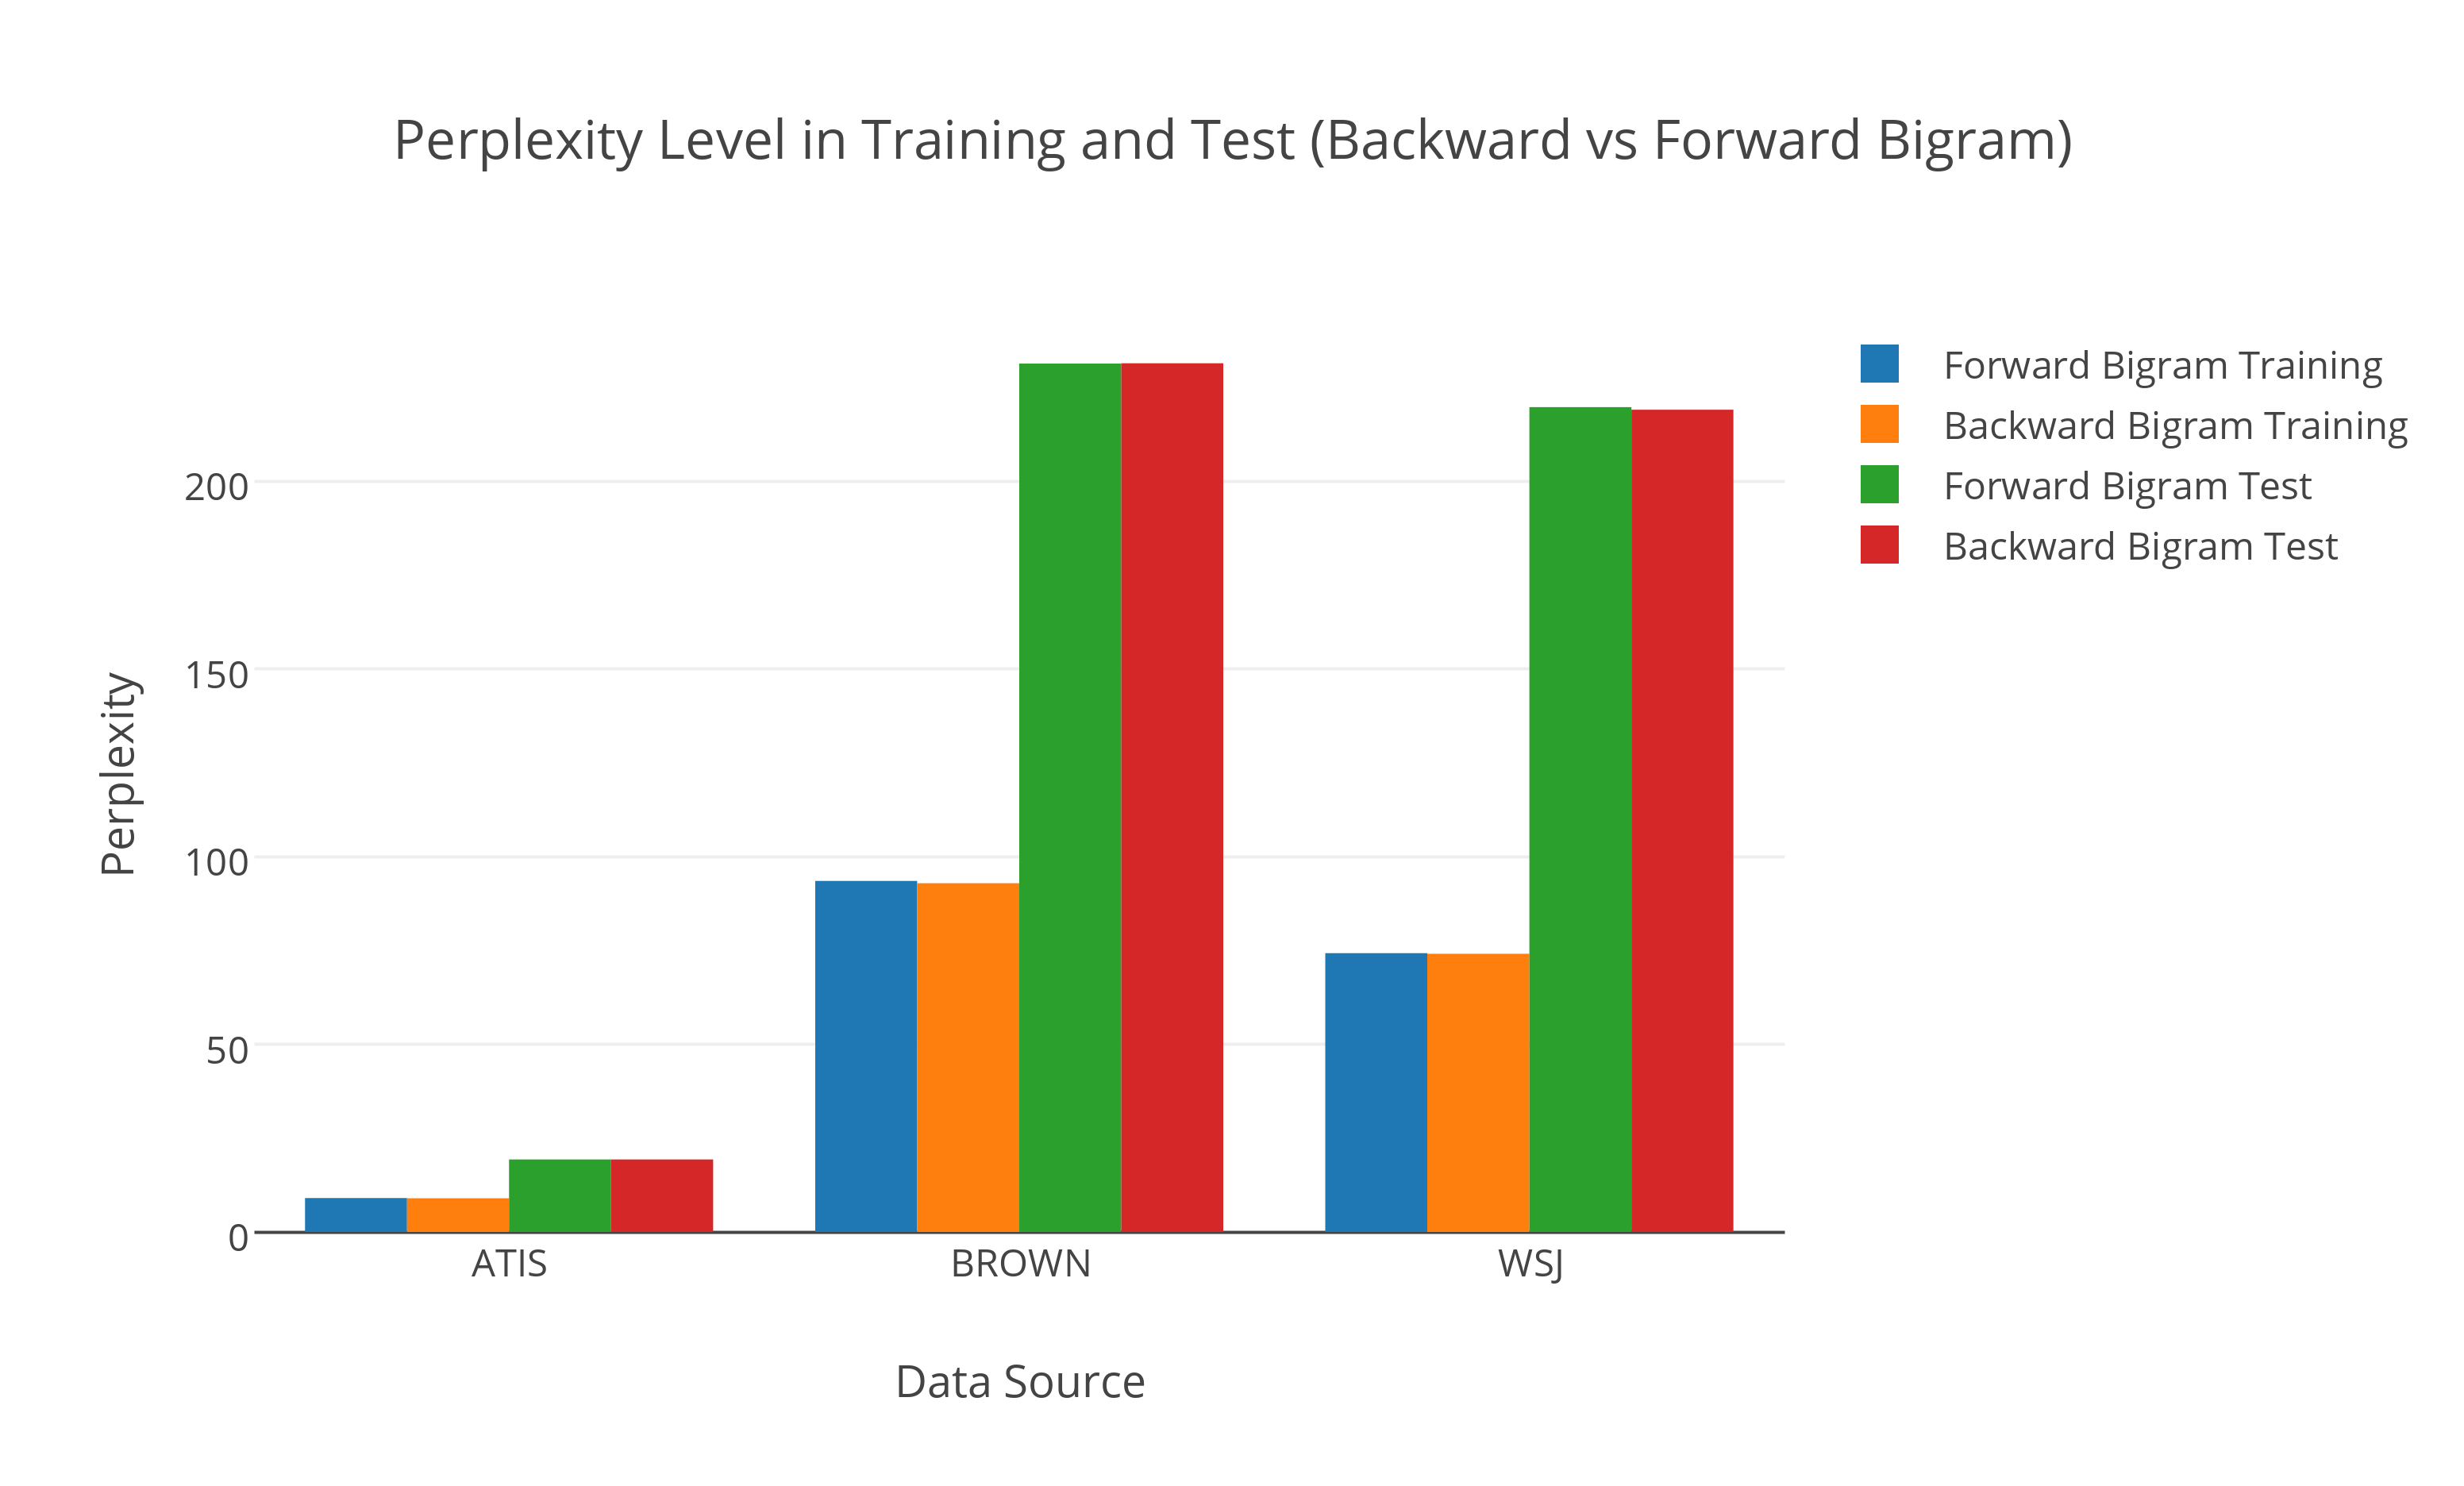
\includegraphics[width=80mm]{perplexity_level_in_training_and_test_backward_vs_forward_bigram.png}%
            \label{fig:left}%
        }\hfill%
        \subfloat[Word Perplexity Results]{%
        	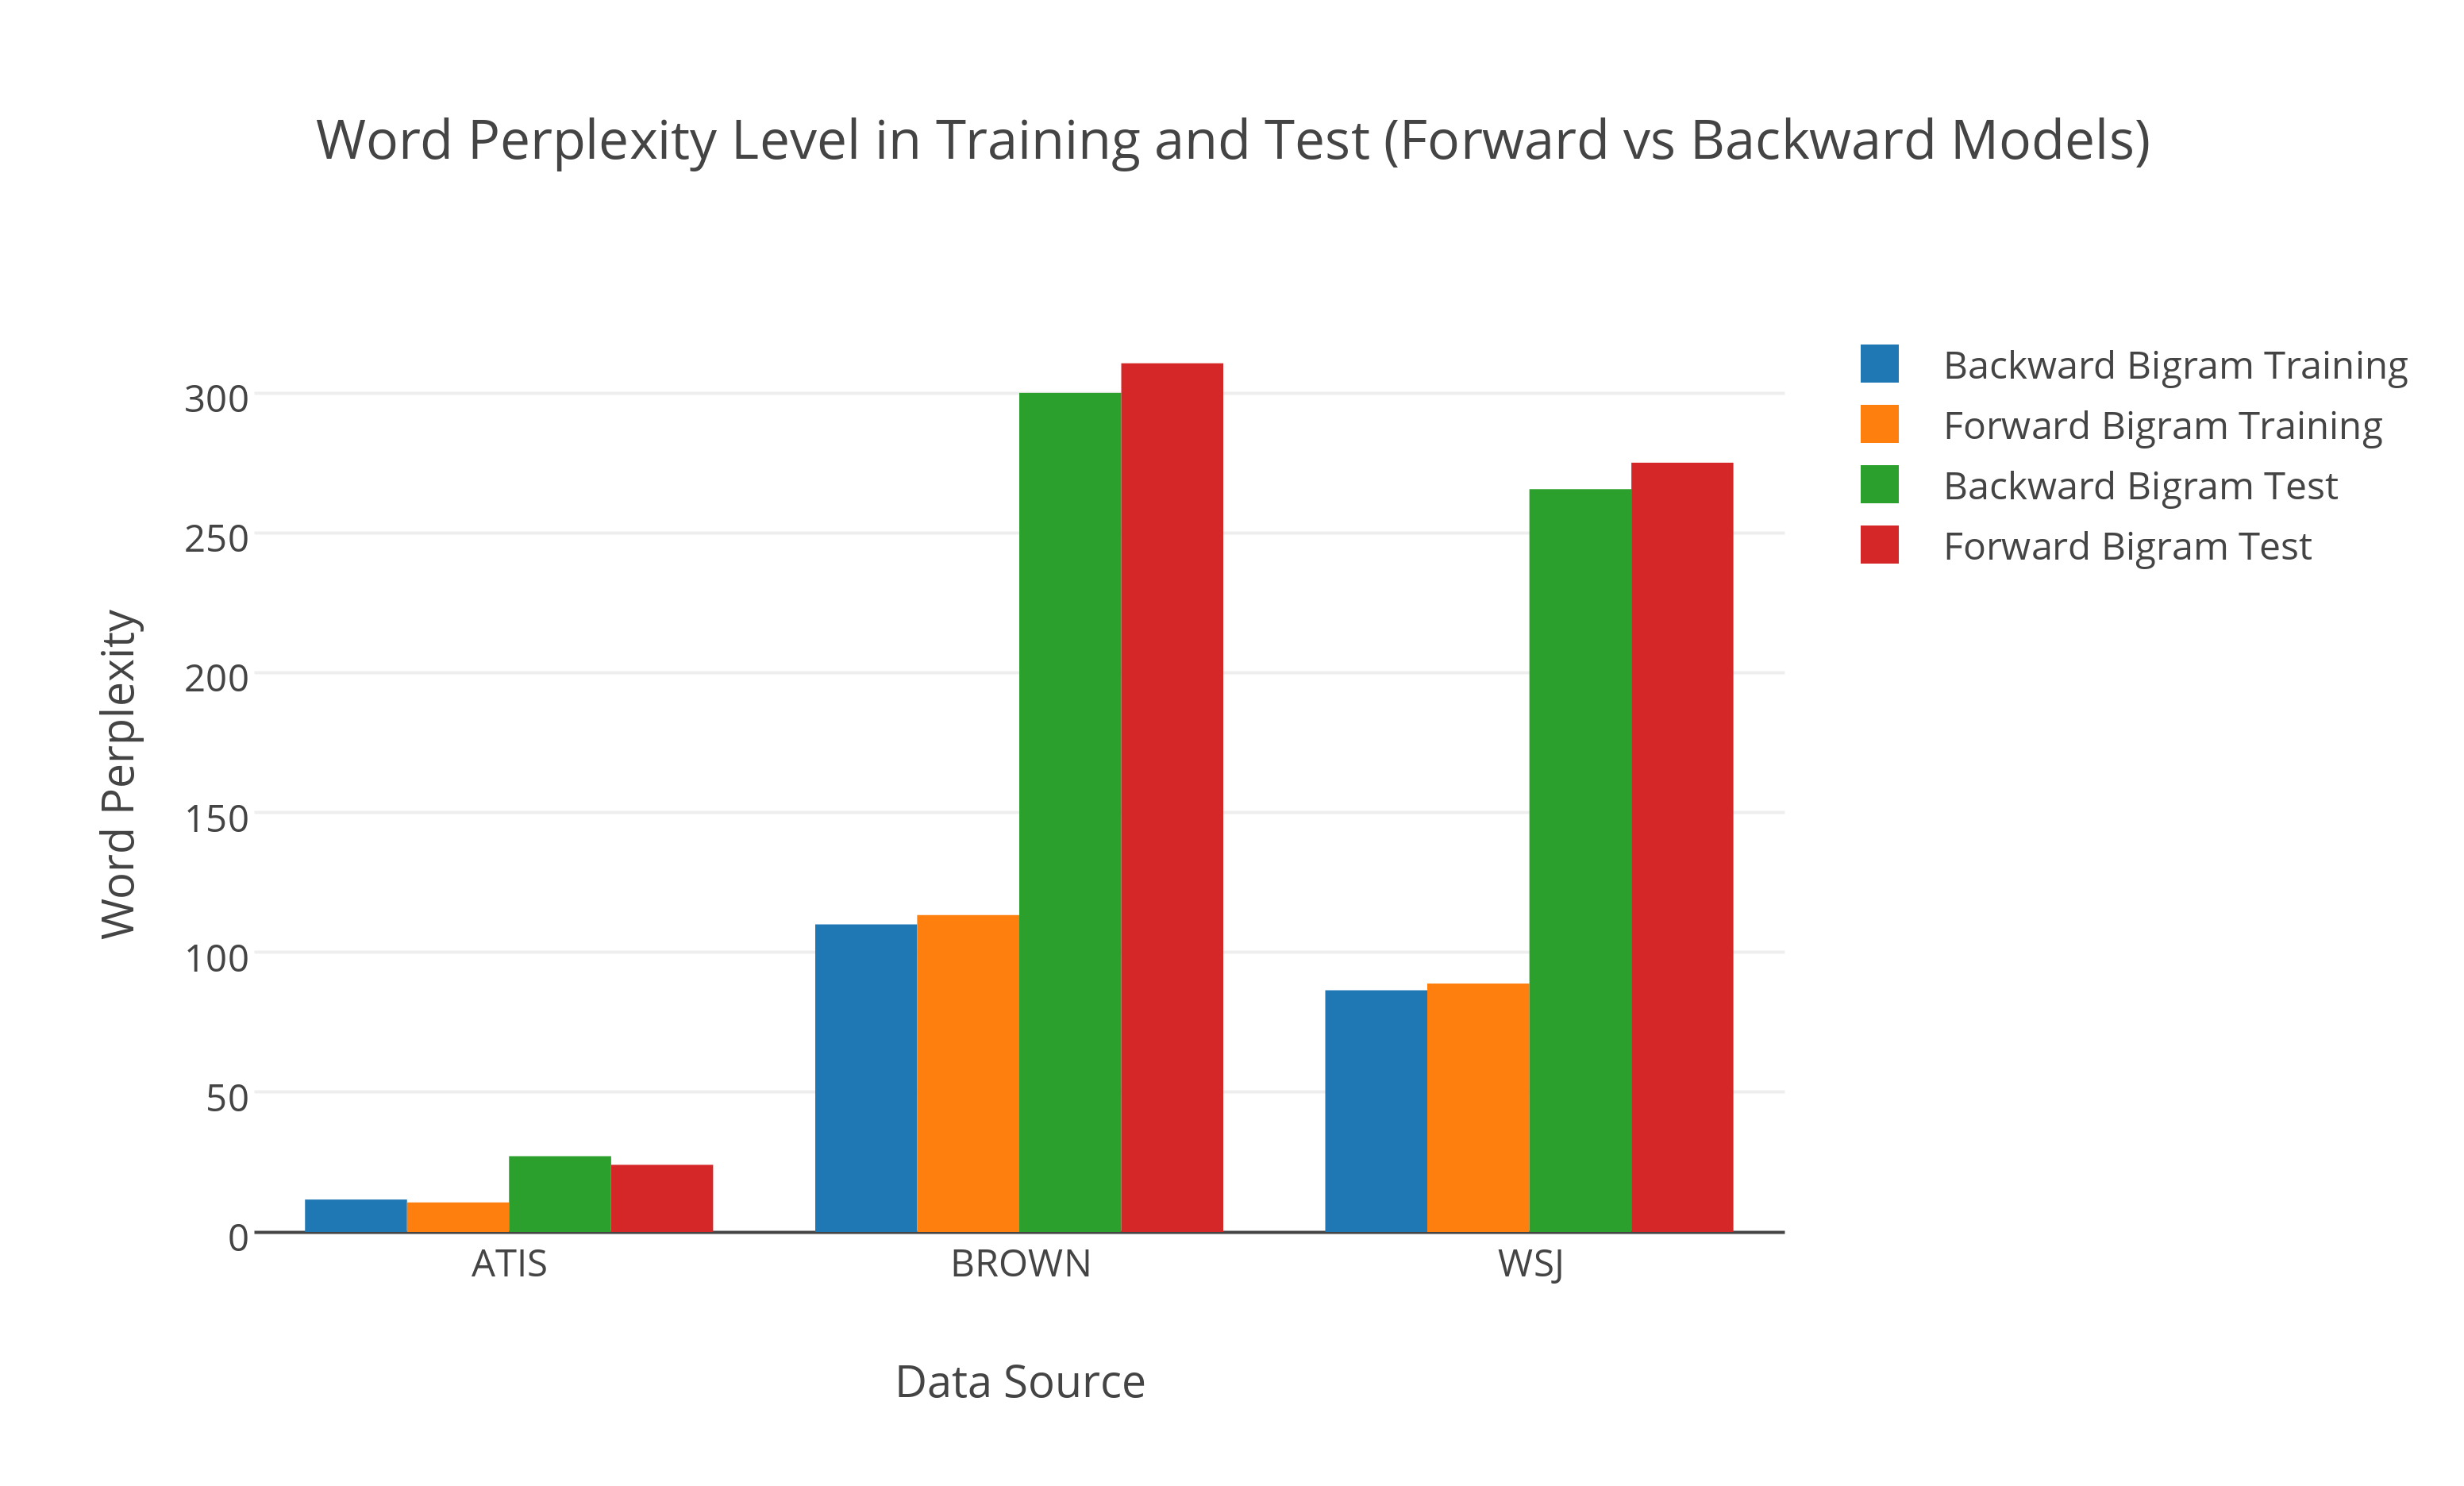
\includegraphics[width=80mm]{word_perplexity_level_in_training_and_test_forward_vs_backward_models__1_.png}%
            \label{fig:right}%
        }
    \caption{\textit{Comparisons of Perplexity and Word Perplexity results between Forward and Backward Bigram}}
    \label{fig:default}
\end{figure}

\begin{table*}[h]
\centering
\caption{\label{tab:widgets} \textit{Perplexity (P) and Word Perplexity (WP) values for the Forward and Backward Bigram models.}}
\begin{tabu}{|c|c|c|c|c|c|c|}
\cline{2-7}
\rowfont{\bfseries}\multicolumn{1}{c}{} & \multicolumn{2}{ |c| }{ATIS} & \multicolumn{2}{ |c| }{Brown} & \multicolumn{2}{ |c| }{WSJ} \\\cline{2-7}
\rowfont{\bfseries} \multicolumn{1}{c}{} & \multicolumn{1}{|c|}{P} & WP & P & WP & P & WP \\\hline
\textbf{Forward Train} & 9.0432 & 10.5920 & 93.5192 & 113.3595 & 74.2680 & 88.8901 \\\hline
\textbf{Backward Train} & 8.9965 & 11.6012 & 92.9093 & 110.0041 & 74.1195 & 86.4558 \\\hline
\textbf{Forward Test} & 19.3414 & 24.0540 & 231.3024 & 310.6674 & 219.7152 & 275.1178 \\\hline
\textbf{Backward Test} & 19.3212 & 27.1135 & 231.3784 & 300.1065 & 219.0260 & 265.6597 \\\hline
\end{tabu}
\end{table*}

Based on the generated results, in neither of the three corpora was there a significant difference in perplexity between the two models. The perplexity results, especially, were nearly identical as both the values in Table 1 as well as Figure 1a indicate. There seems to be a small discrepancy in the Word Perplexity results. Specifically, in the Brown and WSJ datasets, there is a slight decrease in perplexity when using the Backward model versus the Forward model in both the training and test evaluations. However, the differences were slight and less than \(5\%\). In the ATIS data set, however, the perplexity increased by approximately 3 for the test set when using the Backward model instead of the Forward model.

\subsection{Bidirectional Bigram versus Backward and Forward Bigram}

The Bidirectional Bigram model is constructed based on an interpolation of probability values from the Forward and the Backward Bigram models. In my implementation, the higher the interpolation factor, the higher the Forward Bigram model is weighted. The assignment prompt suggests to utilize the interpolation factor of 0.5 for the value of the interpolation factor, incorporating equal influence from both Forward and Bigram models. Table 2 contains the results of the Bidirectional Model at an interpolation factor of 0.5.

\begin{table*}[h]
\centering
\caption{\label{tab:widgets} \textit{Word Perplexity (WP) values for the Forward, Backward, and Bidirectional Bigram (at interpolation value of 0.5) models.}}
\begin{tabu}{|c|c|c|c|c|c|c|}
\cline{2-7}
\rowfont{\bfseries}\multicolumn{1}{c}{} & \multicolumn{2}{ |c| }{ATIS} & \multicolumn{2}{ |c| }{Brown} & \multicolumn{2}{ |c| }{WSJ} \\\cline{2-7}
\rowfont{\bfseries} \multicolumn{1}{c}{} & \multicolumn{1}{|c|}{P} & WP & P & WP & P & WP \\\hline
\textbf{Forward Train} & 9.0432 & 10.5920 & 93.5192 & 113.3595 & 74.2680 & 88.8901 \\\hline
\textbf{Backward Train} & 8.9965 & 11.6012 & 92.9093 & 110.0041 & 74.1195 & 86.4558 \\\hline
\textbf{Bidirectional Train @ .5} & - & 6.9303 & - & 57.0417 & - & 43.7931 \\\hline
\textbf{Forward Test} & 19.3414 & 24.0540 & 231.3024 & 310.6674 & 219.7152 & 275.1178 \\\hline
\textbf{Backward Test} & 19.3212 & 27.1135 & 231.3784 & 300.1065 & 219.0260 & 265.6597 \\\hline
\textbf{Bidirectional Test @ .5} & - & 13.0175 & - & 167.6776 & - & 125.9530 \\\hline
\end{tabu}
\end{table*}

Based on the results in Table 2, the Bidirectional Model at an interpolation factor of 0.5 significantly outperforms the vanilla Forward or Backward Bigram models in all three data sets in both training and test results. For example, there was an approximate \(55\%\) reduction in Word Perplexity for the Bidirectional model when comparing against the Forward model in the WSJ data set test results. Similarly, there was an approximate \(50\%\) reduction in Word Perplexity for the Bidirectional model when comparing against the Backward model in the WSJ data set training results.

For the sake of completeness, I also tried to gauge the performance of the Bidirectional model at various interpolation factor values, starting from 0.0 to 1.0 with a step size of 0.1. The results are captured in the graphs in Figure 2.

\begin{figure}%
	\centering
        \subfloat[Word Perplexity Results for ATIS dataset]{%
        	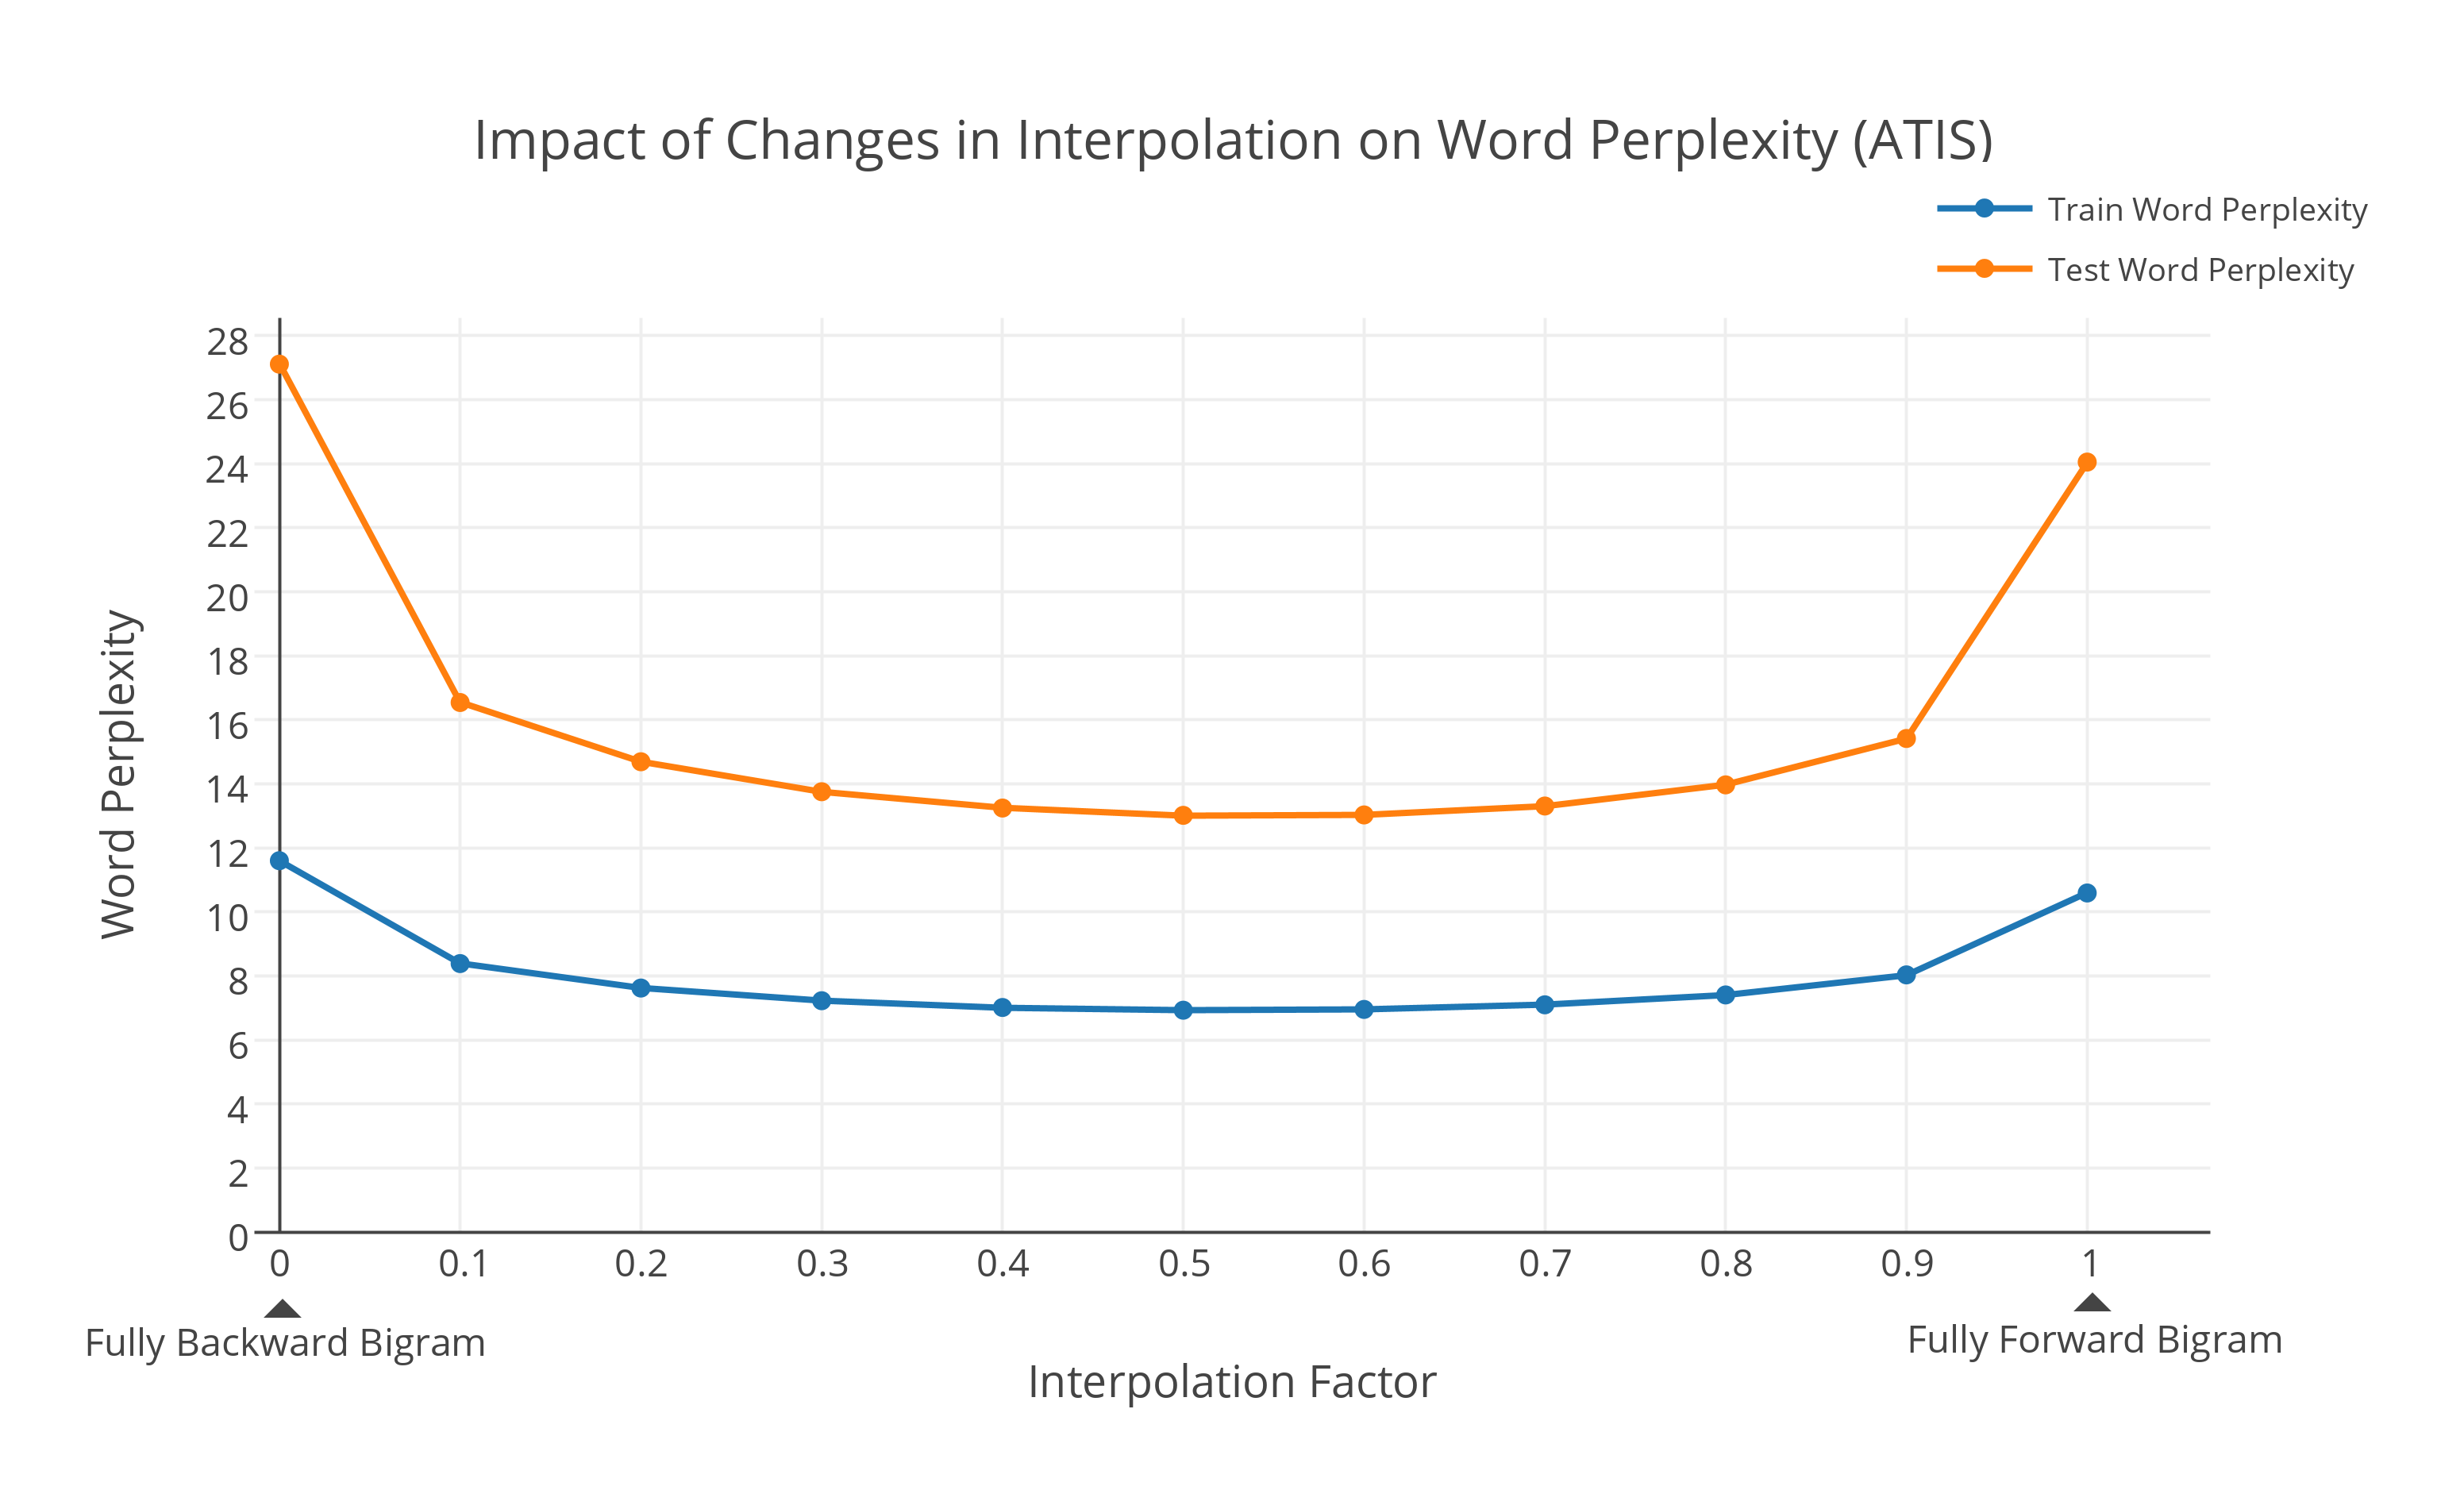
\includegraphics[width=110mm]{impact_of_changes_in_interpolation_on_word_perplexity_atis.png}%
            \label{fig:right}%
        }\hfill%
        \subfloat[Word Perplexity Results for Brown dataset]{%
        	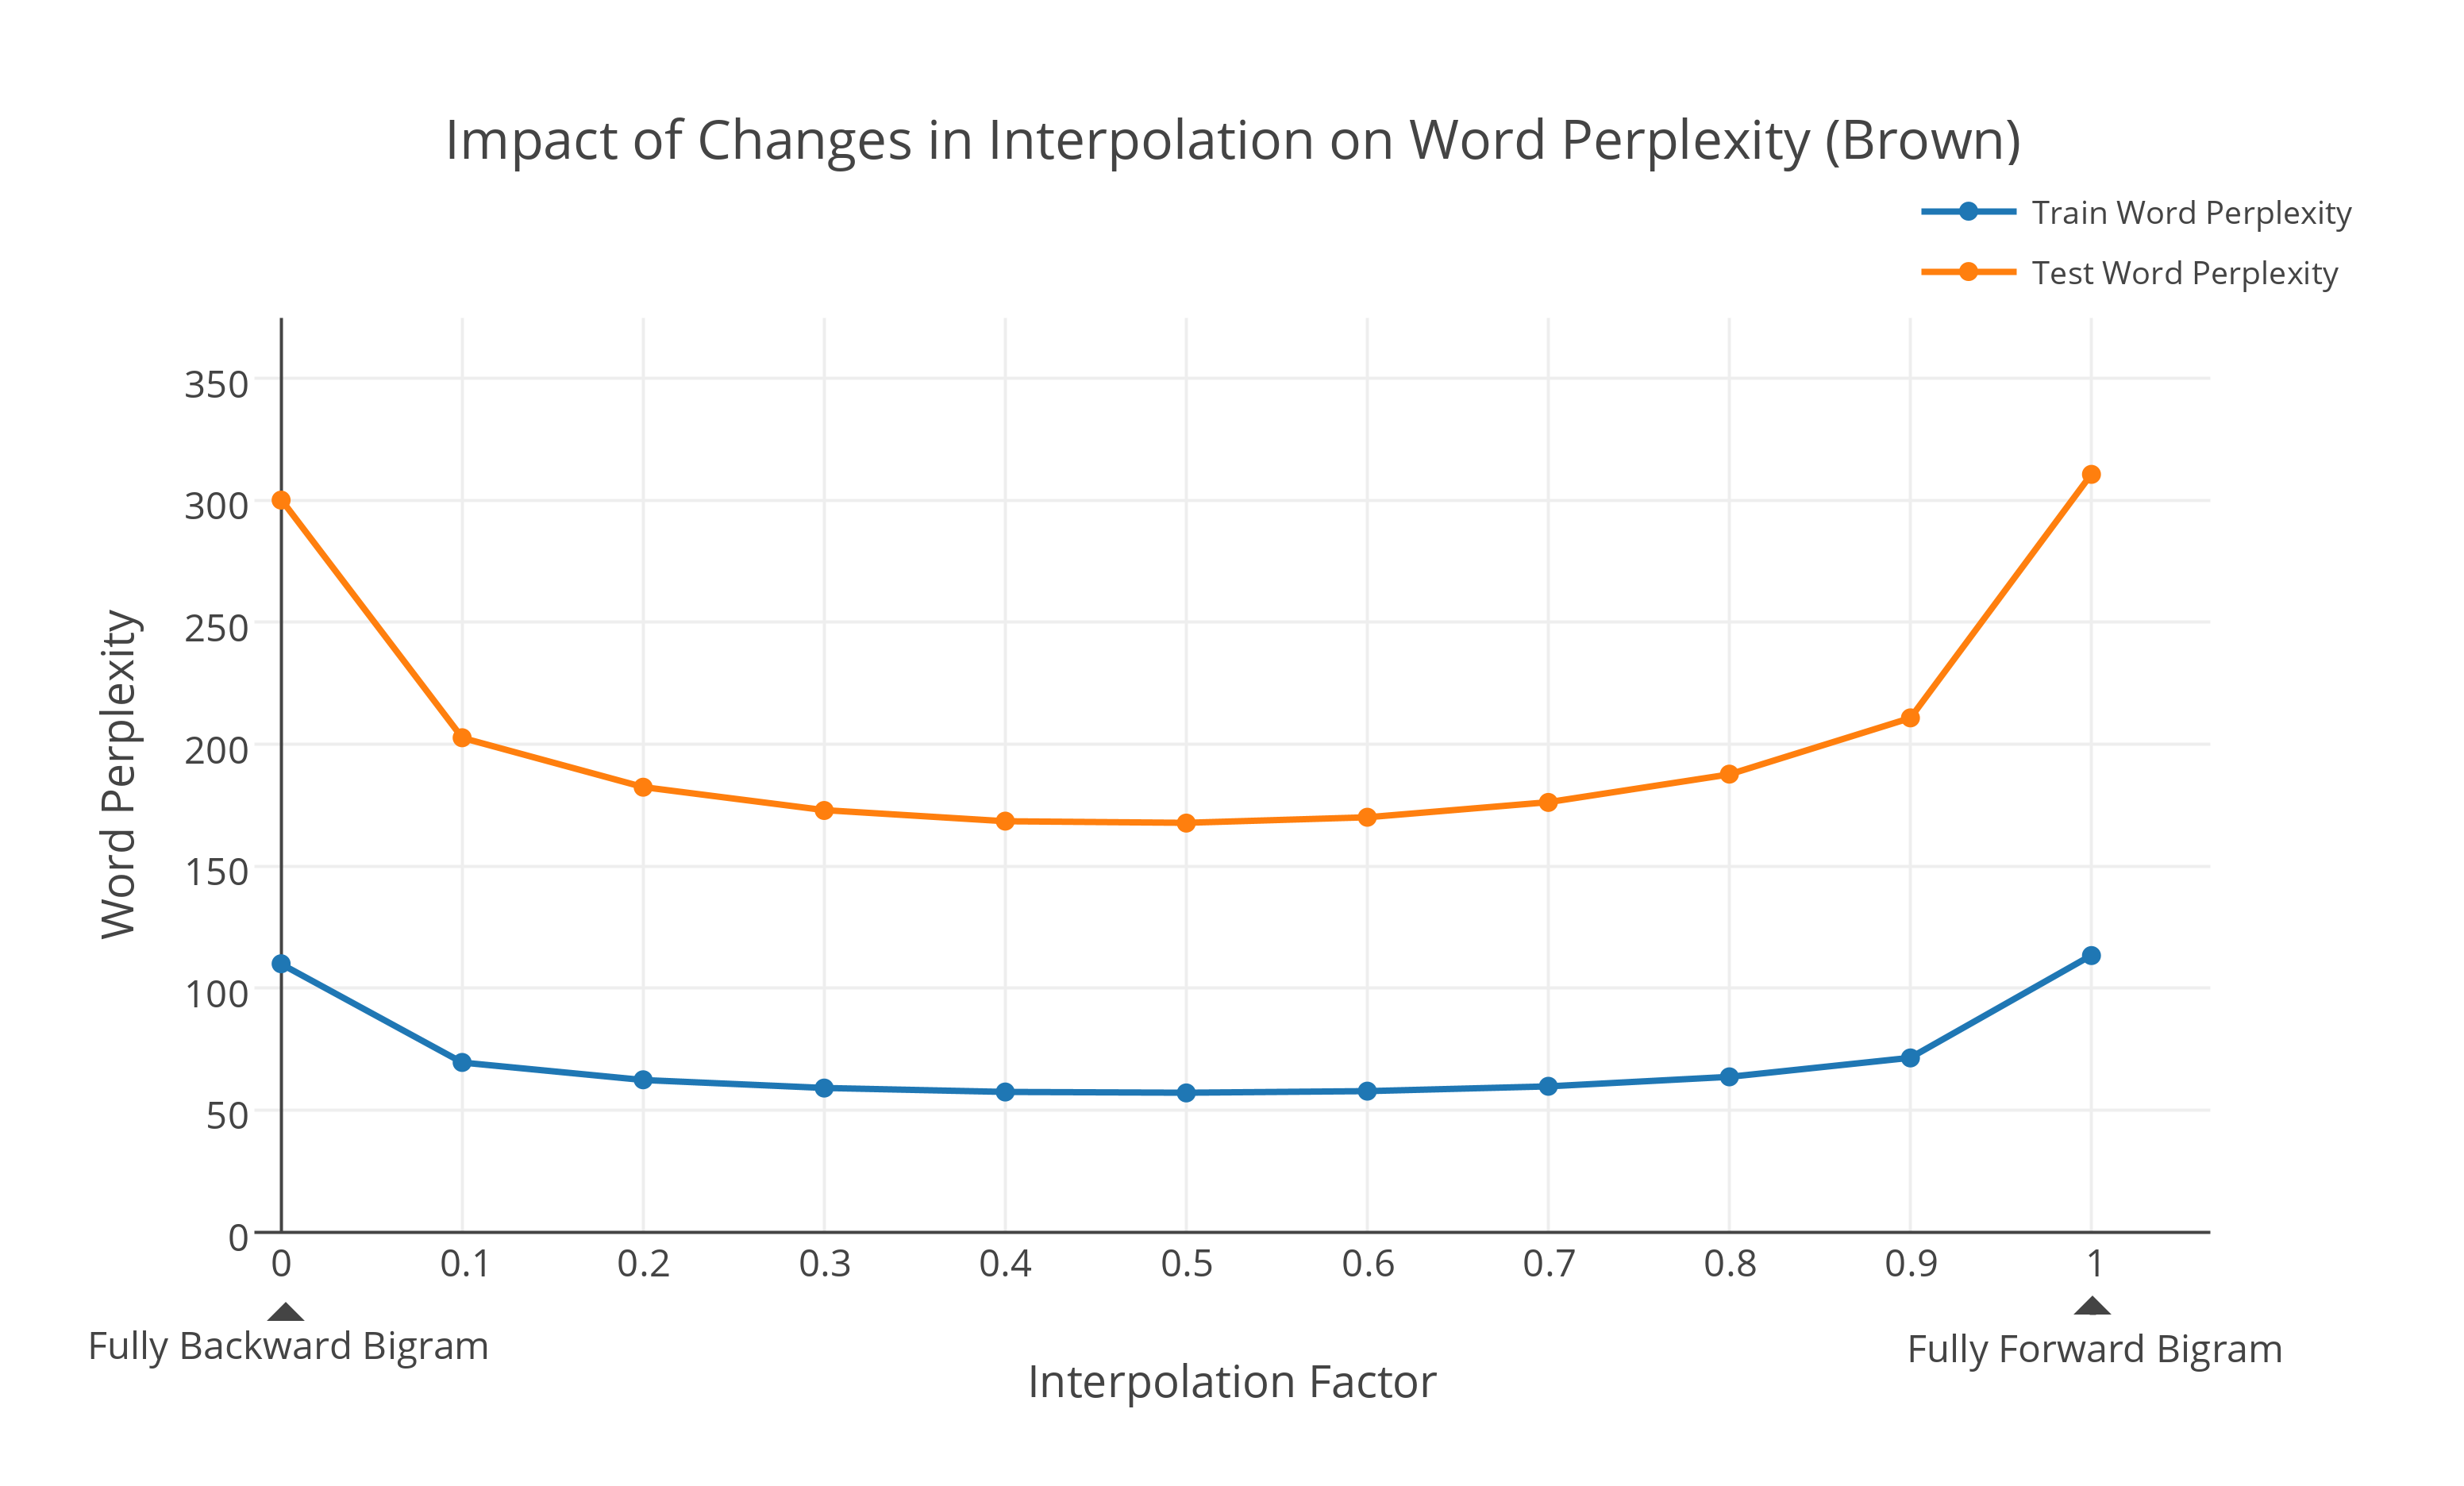
\includegraphics[width=110mm]{impact_of_changes_in_interpolation_on_word_perplexity_brown.png}%
            \label{fig:right}%
        }\hfill%
        \subfloat[Word Perplexity Results for WSJ dataset]{%
        	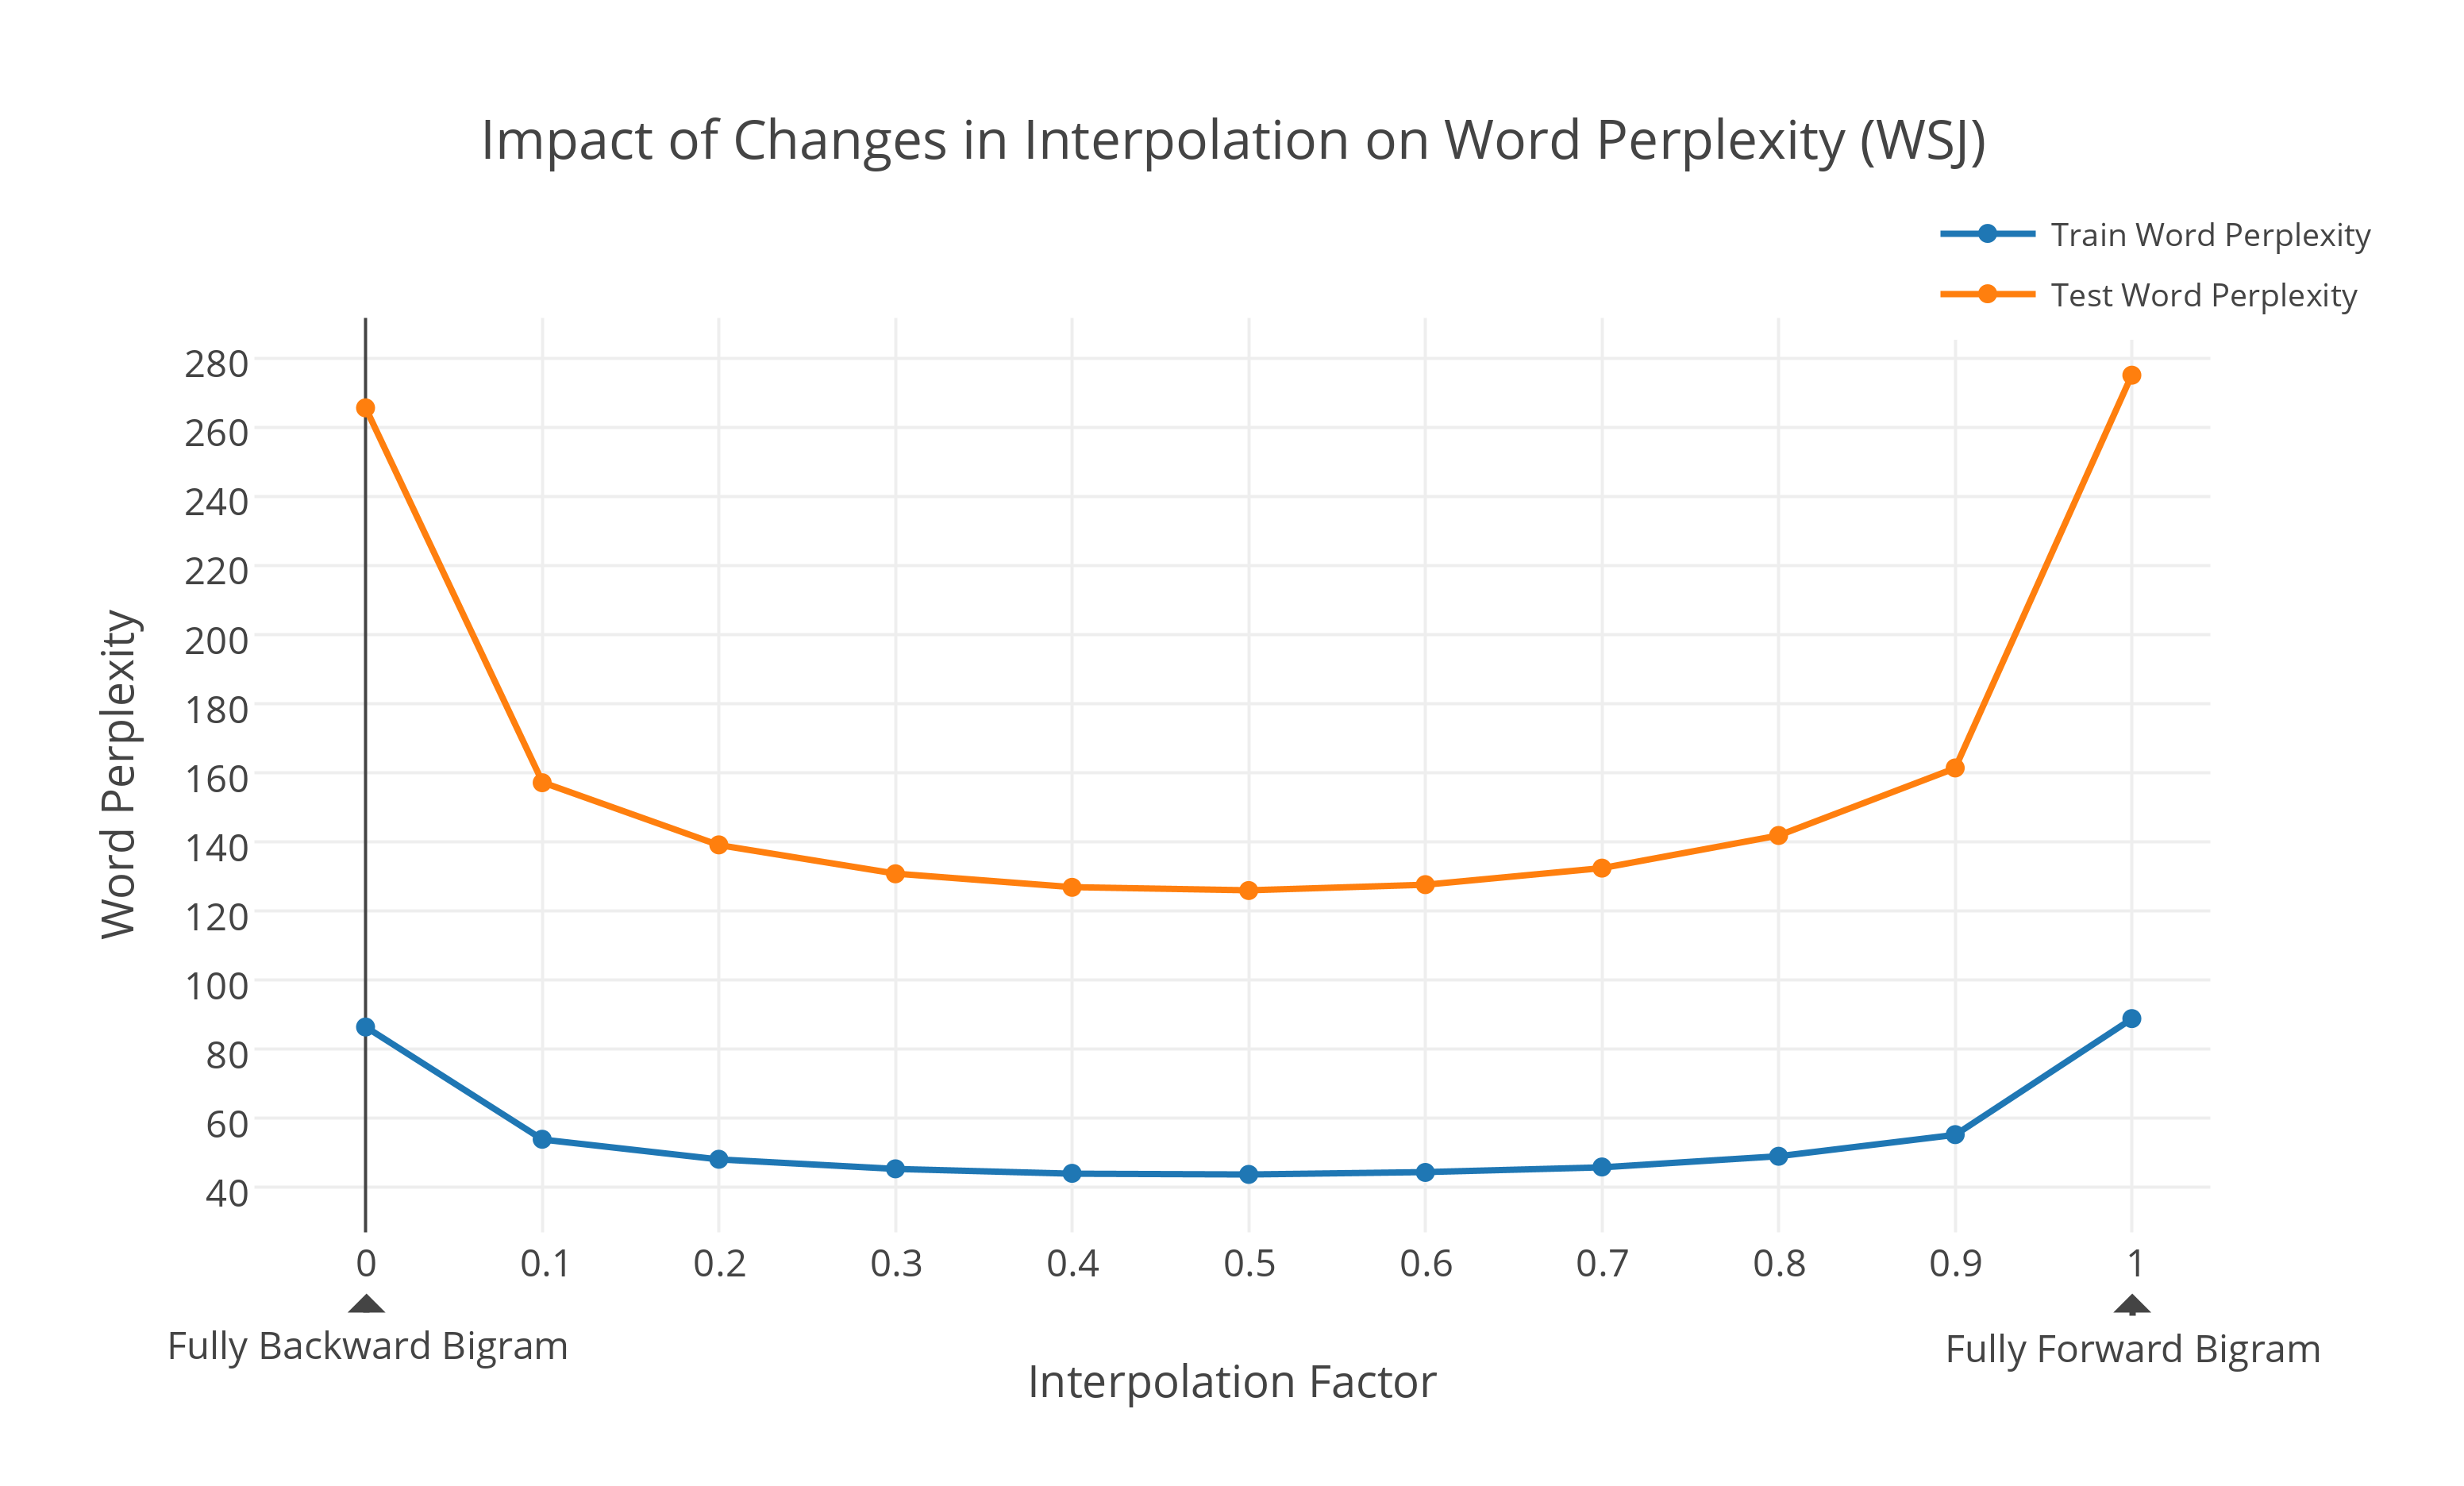
\includegraphics[width=110mm]{impact_of_changes_in_interpolation_on_word_perplexity_wsj.png}%
            \label{fig:right}%
        }
    \caption{\textit{Word Perplexity results for the Bidirectional Bigram model at various interpolation factor values.}}
    \label{fig:default}
\end{figure}

Note that an interpolation value of 0.0 is the equivalent to the Backward Bigram model and an interpolation value of 1.0 is the equivalent to the Forward Bigram model. Based on the curvature of the graphs in Figure 2, for each of the data sets, it seems that any degree of combining the Backward and Forward Bigram models provides a superior model to the Forward Bigram (i.e. at 1.0) or the Backward Bigram (i.e. at 0.0) models by themselves. The curvatures all achieve their lowest point at an interpolation factor of 0.5 and, minor deviations aside, are fairly symmetric around the point of 0.5.  

\section{Discussion}

The following subsections provide a discussion of the results presented in Section 3.

\subsection{Backward Context versus Forward Context}

The Backward Bigram model did not provide a significant improvement or detriment in statistically modeling the language data in the three data sets, as seen in Figure 1 and Table 1. The differences in Perplexity and Word Perplexity observed in Figure 1 and Table 1 are not necessarily significant differences, given how small of an improvement or detriment is observed. Intuitively, I did not expect a significant improvement through resorting to the Backward Bigram model. In general, specific tokens might be better estimated by inspecting the tokens proceeding the token. However, the data sets used did not predominantly contain such tokens and the language itself doesn't hold any similar property to give any reason to intuitively assume that a Backward Bigram model might perform better than a Forward Bigram model. If that property consistently held in a data set of a particular language, then the Backward Bigram model can consistently be expected to outperform the Forward Bigram model. In this scenario, with the ATIS, Brown, and WSJ data sets, there are likely some tokens that are better modeled with past data and other tokens which are better modeled with future data. Given that the presence of tokens that favor either the Forward doesn't dominate those that favor the Backward model and vice-versa, I intuitively expected the Backward and Forward Bigram models to perform approximately equally well.

The shape of the curvature in the graphs in Figure 2 supports this notion. In general, the curvature in the graphs is fairly symmetrical around the interpolation point of 0.5, which is the point of balance between a fully Forward Bigram model and a fully Backward Bigram model. If the Backward or the Forward Bigram had better performance than the other, the curvature would likely have been more skewed towards the the model that performed better. Therefore, the fact that the curvature is symmetric and the deepest valley exists at the interpolation point of 0.5 provides further evidence that, in the context of the language and the data sets used, the Backward and Forward Bigram models were more or less equally effective, barring slight differences.

The novelty of the Backward Bigram model stems from the fact that the context used for each token is in the future tokens of a sentence rather than the past. As a result, the Backward Bigram model still shares the problems that plague the Forward Bigram model. For example, the Backward Bigram model still suffers from the long distance context problem that plagued the Forward Bigram model. Although the Backward Bigram model uses the context of a word in the future, words or context that exist a longer distance from the current position are still not adequately captured. 

\subsection{Impact of Extra Context}

An interpolation factor value of 0.0 represents the equivalent of a fully Backward Bigram model. In Figure 2, the drop in Word Perplexity from interpolation factor constant 0.0 to 0.1 is sharp. This rate of drop decreases significantly after this point and the pattern is observable in all three graphs. A key observation is that the sharpest decrease occurs when the context of the Forward Bigram model is begun to be added to the Backward Bigram model. In other words, the smallest bit of extra context added to the standalone Backward Bigram model provides a significant boost in both training and test result performance.

Similarly, in all of the curves, the rate of increase in Word Perplexity culminates in a sharp increase at the transition from interpolation value 0.9 to 1.0. This represents the point where the model loses all context from the Backward Bigram model and becomes the equivalent of a fully Forward Bigram model. As before, the key observation here is that once the last bit of context from the Backward Bigram model was no longer present, the overall model performed much worse.

The observations noted above imply that the extra context added by including a second model is the reason that the Bidirectional Bigram model performs significantly better than the Forward or Backward Bigram models. Intuitively, the phenomenon makes sense due to the same reasoning behind the intuitive expectation for a Forward Trigram model to outperform a Forward Bigram model - additional context. In the fully Forward or fully Backward Bigram models, the only available context is a single word in the past (i.e. the Forward Bigram model) or a single word in the future (i.e. the Backward Bigram model). By combining the contexts from both the Backward and Forward Bigram models, the Bidirectional Bigram model has the combined context of a word in the past as well as a word in the future. The additional context can make it easier for the Bidirectional Bigram model to better statistically model the language.

However, though extra context is present, the Bidirectional Bigram model, as constructed, still suffers from the long distance dependencies problem as the standard Forward Bigram model does. Though the additional context provides more information in smaller distances and contexts, longer distance contexts still might pose problems for language models built on this construction of the Bidirectional Bigram model.

\subsection{Interpolation Sweet Spot}

Based on Figure 1, in each of the data sets as well as in both training and test, the best performing bidirectional model utilized an interpolation factor of 0.5, essentially providing equal weight to both Forward and Backward Bigram models. Intuitively, the performance makes sense. Based on the reasoning above, the Forward and Backward Bigram models were expected to perform approximately equally well on the data sets utilized in this assignment. Therefore, it makes sense to utilize an interpolation factor of 0.5, providing equal emphasis to the predictions from both models. As mentioned before, this is reaffirmed by the fact that the curvature of the graphs in Figure 2 are symmetric around the 0.5 value.

However, I stop short of declaring the halfway mark as the best interpolation factor for all possible data sets. The actual interpolation factor is likely dependent on the actual language and the data set involved. For example, if a particular kind of language or data set exists such that there it's easier to predict a word given future context, the Backward Bigram model would perform better than the Forward Bigram model and as a result, the interpolation factor would need to be set to prioritize the the Backward Bigram model more. A similar argument exists for an Forward Bigram model analogue. Therefore, deciding the best interpolation factor is dependent on:

\begin{itemize}
\item Being able to evaluate the performance of the Backward and Forward Bigram models.
\item Simply trying out various interpolation factors based on the intuition of how well suited a Backward or Forward model is to the current data set and use case.

\end{itemize}
\end{document}